\documentclass[tikz, border=6pt]{standalone}
\IfFileExists{lmodern.sty}{\usepackage[T1]{fontenc}\usepackage{lmodern}}{}
\usepackage{amsmath,amssymb,bm}
\usepackage[scaled=0.95]{helvet}
\usetikzlibrary{arrows.meta}
\definecolor{Blue}{HTML}{3A76D8}
\definecolor{Teal}{HTML}{16A394}
\definecolor{Orange}{HTML}{EE8133}
\definecolor{Gray}{HTML}{6B7280}
\definecolor{Ink}{HTML}{1F2937}
\colorlet{activation}{Teal}
\begin{document}
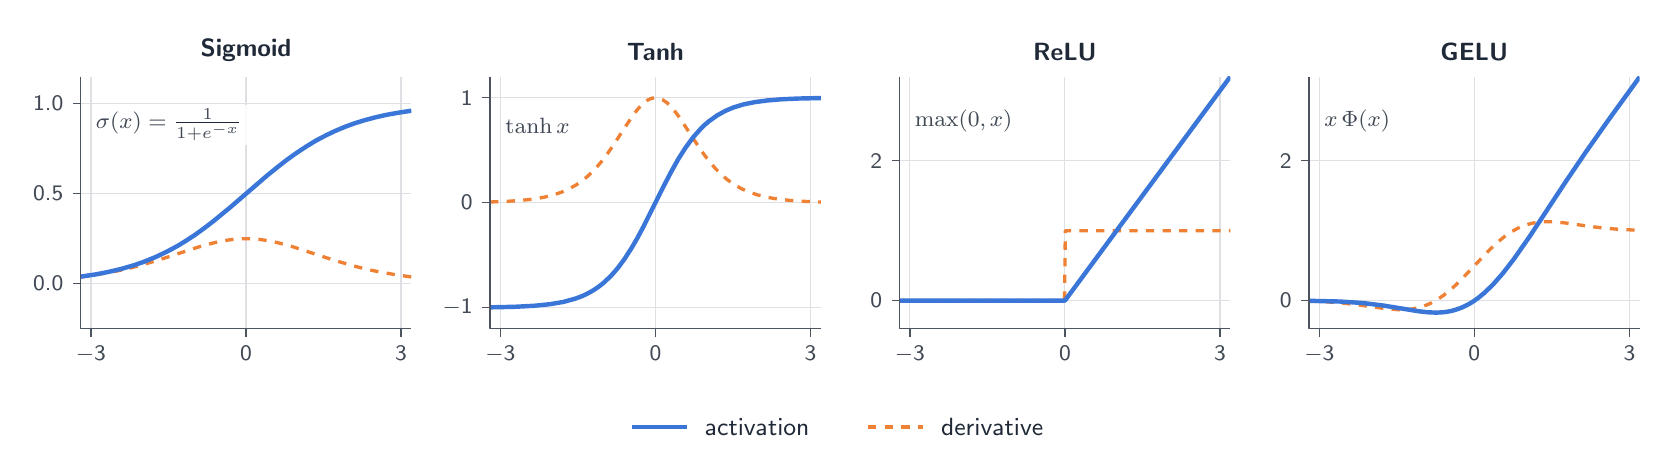
\begin{tikzpicture}[color=Ink, execute at begin picture={\sffamily}, line width=0.6pt, >={Stealth[length=5.5pt, width=4pt, inset=1.2pt]}, line join=round]
  % axes ax1
  \draw[Gray!22, line width=0.4pt] (0.131,0) -- (0.131,3.2) (2.1,0) -- (2.1,3.2) (4.069,0) --
      (4.069,3.2) (0,0.571) -- (4.2,0.571) (0,1.714) -- (4.2,1.714) (0,2.857) -- (4.2,2.857);
  \begin{scope}
    \clip (0,0) rectangle (4.2,3.2);
    \draw[dashed, color=Orange, line width=1.2pt] (0,0.657) -- (0.179,0.682) -- (0.358,0.712) --
        (0.526,0.746) -- (0.684,0.784) -- (0.968,0.865) -- (1.505,1.04) -- (1.705,1.094) --
        (1.811,1.116) -- (1.905,1.13) -- (2,1.14) -- (2.095,1.143) -- (2.189,1.14) -- (2.284,1.132) --
        (2.389,1.116) -- (2.495,1.094) -- (2.695,1.04) -- (3.232,0.865) -- (3.516,0.784) --
        (3.674,0.746) -- (3.842,0.712) -- (4.021,0.682) -- (4.2,0.657);
    \draw[color=Blue, line width=1.6pt] (0,0.661) -- (0.189,0.689) -- (0.358,0.722) -- (0.516,0.759) --
        (0.674,0.805) -- (0.821,0.856) -- (0.958,0.913) -- (1.095,0.978) -- (1.232,1.052) --
        (1.337,1.116) -- (1.453,1.192) -- (1.568,1.275) -- (1.684,1.364) -- (1.895,1.537) --
        (2.368,1.945) -- (2.495,2.048) -- (2.621,2.146) -- (2.747,2.236) -- (2.874,2.319) --
        (2.989,2.389) -- (3.116,2.456) -- (3.232,2.511) -- (3.358,2.564) -- (3.484,2.61) --
        (3.611,2.649) -- (3.747,2.685) -- (3.884,2.716) -- (4.042,2.744) -- (4.2,2.768);
  \end{scope}
  \draw[Ink!80, line width=0.5pt] (0,3.2) -- (0,0) -- (4.2,0);
  \draw[Ink!80, line width=0.5pt] (0.131,0) -- (0.131,-0.1) (2.1,0) -- (2.1,-0.1) (4.069,0) --
      (4.069,-0.1) (0,0.571) -- (-0.1,0.571) (0,1.714) -- (-0.1,1.714) (0,2.857) -- (-0.1,2.857);
  \node[anchor=north, font=\footnotesize, text=Ink!85, inner sep=2pt] (ax1-xt0) at (0.131,-0.14) {$-$3};
  \node[anchor=north, font=\footnotesize, text=Ink!85, inner sep=2pt] (ax1-xt1) at (2.1,-0.14) {0};
  \node[anchor=north, font=\footnotesize, text=Ink!85, inner sep=2pt] (ax1-xt2) at (4.069,-0.14) {3};
  \node[anchor=east, font=\footnotesize, text=Ink!85, inner sep=2pt] (ax1-yt0) at (-0.14,0.571) {0.0};
  \node[anchor=east, font=\footnotesize, text=Ink!85, inner sep=2pt] (ax1-yt1) at (-0.14,1.714) {0.5};
  \node[anchor=east, font=\footnotesize, text=Ink!85, inner sep=2pt] (ax1-yt2) at (-0.14,2.857) {1.0};
  \node[anchor=north west, font=\footnotesize, fill=white, fill opacity=0.85, inner sep=1.5pt] at (0.131,2.857) {$\sigma(x)=\frac{1}{1+e^{-x}}$};
  \node[anchor=south, font=\small\bfseries, inner sep=4pt, align=center] at (2.1,3.25) {Sigmoid};
  % axes ax2
  \draw[Gray!22, line width=0.4pt] (5.331,0) -- (5.331,3.2) (7.3,0) -- (7.3,3.2) (9.269,0) --
      (9.269,3.2) (5.2,0.267) -- (9.4,0.267) (5.2,1.6) -- (9.4,1.6) (5.2,2.933) -- (9.4,2.933);
  \begin{scope}
    \clip (5.2,0) rectangle (9.4,3.2);
    \draw[dashed, color=Orange, line width=1.2pt] (5.2,1.609) -- (5.411,1.617) -- (5.589,1.629) --
        (5.737,1.645) -- (5.874,1.667) -- (6,1.698) -- (6.105,1.733) -- (6.2,1.774) -- (6.295,1.827) --
        (6.379,1.886) -- (6.453,1.948) -- (6.537,2.032) -- (6.611,2.118) -- (6.674,2.2) -- (6.747,2.304)
        -- (7,2.689) -- (7.053,2.76) -- (7.095,2.811) -- (7.147,2.864) -- (7.2,2.903) -- (7.253,2.926)
        -- (7.295,2.933) -- (7.337,2.929) -- (7.389,2.909) -- (7.442,2.873) -- (7.495,2.822) --
        (7.547,2.76) -- (7.6,2.689) -- (7.853,2.304) -- (7.926,2.2) -- (7.989,2.118) -- (8.063,2.032) --
        (8.147,1.948) -- (8.221,1.886) -- (8.305,1.827) -- (8.4,1.774) -- (8.495,1.733) -- (8.6,1.698)
        -- (8.726,1.667) -- (8.863,1.645) -- (9.011,1.629) -- (9.189,1.617) -- (9.4,1.609);
    \draw[color=Blue, line width=1.6pt] (5.2,0.271) -- (5.516,0.278) -- (5.758,0.291) -- (5.958,0.311)
        -- (6.126,0.339) -- (6.274,0.379) -- (6.347,0.405) -- (6.411,0.433) -- (6.474,0.466) --
        (6.526,0.497) -- (6.589,0.541) -- (6.642,0.583) -- (6.737,0.673) -- (6.821,0.769) --
        (6.905,0.883) -- (7,1.03) -- (7.074,1.158) -- (7.147,1.295) -- (7.4,1.802) -- (7.495,1.984) --
        (7.589,2.153) -- (7.684,2.302) -- (7.779,2.431) -- (7.874,2.538) -- (7.926,2.589) --
        (7.979,2.634) -- (8.084,2.709) -- (8.189,2.767) -- (8.295,2.811) -- (8.421,2.849) --
        (8.558,2.877) -- (8.716,2.898) -- (8.895,2.913) -- (9.116,2.923) -- (9.4,2.929);
  \end{scope}
  \draw[Ink!80, line width=0.5pt] (5.2,3.2) -- (5.2,0) -- (9.4,0);
  \draw[Ink!80, line width=0.5pt] (5.331,0) -- (5.331,-0.1) (7.3,0) -- (7.3,-0.1) (9.269,0) --
      (9.269,-0.1) (5.2,0.267) -- (5.1,0.267) (5.2,1.6) -- (5.1,1.6) (5.2,2.933) -- (5.1,2.933);
  \node[anchor=north, font=\footnotesize, text=Ink!85, inner sep=2pt] (ax2-xt0) at (5.331,-0.14) {$-$3};
  \node[anchor=north, font=\footnotesize, text=Ink!85, inner sep=2pt] (ax2-xt1) at (7.3,-0.14) {0};
  \node[anchor=north, font=\footnotesize, text=Ink!85, inner sep=2pt] (ax2-xt2) at (9.269,-0.14) {3};
  \node[anchor=east, font=\footnotesize, text=Ink!85, inner sep=2pt] (ax2-yt0) at (5.06,0.267) {$-$1};
  \node[anchor=east, font=\footnotesize, text=Ink!85, inner sep=2pt] (ax2-yt1) at (5.06,1.6) {0};
  \node[anchor=east, font=\footnotesize, text=Ink!85, inner sep=2pt] (ax2-yt2) at (5.06,2.933) {1};
  \node[anchor=north west, font=\footnotesize, fill=white, fill opacity=0.85, inner sep=1.5pt] at (5.331,2.733) {$\tanh x$};
  \node[anchor=south, font=\small\bfseries, inner sep=4pt, align=center] at (7.3,3.25) {Tanh};
  % axes ax3
  \draw[Gray!22, line width=0.4pt] (10.531,0) -- (10.531,3.2) (12.5,0) -- (12.5,3.2) (14.469,0) --
      (14.469,3.2) (10.4,0.356) -- (14.6,0.356) (10.4,2.133) -- (14.6,2.133);
  \begin{scope}
    \clip (10.4,0) rectangle (14.6,3.2);
    \draw[dashed, color=Orange, line width=1.2pt] (10.4,0.356) -- (12.495,0.356) -- (12.505,1.244) --
        (14.6,1.244);
    \draw[color=Blue, line width=1.6pt] (10.4,0.356) -- (12.495,0.356) -- (12.505,0.363) -- (14.6,3.2);
  \end{scope}
  \draw[Ink!80, line width=0.5pt] (10.4,3.2) -- (10.4,0) -- (14.6,0);
  \draw[Ink!80, line width=0.5pt] (10.531,0) -- (10.531,-0.1) (12.5,0) -- (12.5,-0.1) (14.469,0) --
      (14.469,-0.1) (10.4,0.356) -- (10.3,0.356) (10.4,2.133) -- (10.3,2.133);
  \node[anchor=north, font=\footnotesize, text=Ink!85, inner sep=2pt] (ax3-xt0) at (10.531,-0.14) {$-$3};
  \node[anchor=north, font=\footnotesize, text=Ink!85, inner sep=2pt] (ax3-xt1) at (12.5,-0.14) {0};
  \node[anchor=north, font=\footnotesize, text=Ink!85, inner sep=2pt] (ax3-xt2) at (14.469,-0.14) {3};
  \node[anchor=east, font=\footnotesize, text=Ink!85, inner sep=2pt] (ax3-yt0) at (10.26,0.356) {0};
  \node[anchor=east, font=\footnotesize, text=Ink!85, inner sep=2pt] (ax3-yt1) at (10.26,2.133) {2};
  \node[anchor=north west, font=\footnotesize, fill=white, fill opacity=0.85, inner sep=1.5pt] at (10.531,2.844) {$\max(0, x)$};
  \node[anchor=south, font=\small\bfseries, inner sep=4pt, align=center] at (12.5,3.25) {ReLU};
  % axes ax4
  \draw[Gray!22, line width=0.4pt] (15.731,0) -- (15.731,3.2) (17.7,0) -- (17.7,3.2) (19.669,0) --
      (19.669,3.2) (15.6,0.356) -- (19.8,0.356) (15.6,2.133) -- (19.8,2.133);
  \begin{scope}
    \clip (15.6,0) rectangle (19.8,3.2);
    \draw[dashed, color=Orange, line width=1.2pt] (15.6,0.35) -- (15.821,0.341) -- (16.021,0.326) --
        (16.211,0.304) -- (16.558,0.256) -- (16.716,0.242) -- (16.811,0.242) -- (16.895,0.248) --
        (16.979,0.264) -- (17.063,0.288) -- (17.147,0.324) -- (17.232,0.371) -- (17.316,0.429) --
        (17.4,0.497) -- (17.474,0.565) -- (17.547,0.638) -- (17.895,1.004) -- (17.989,1.093) --
        (18.074,1.163) -- (18.168,1.229) -- (18.253,1.276) -- (18.337,1.312) -- (18.432,1.339) --
        (18.495,1.35) -- (18.568,1.357) -- (18.642,1.359) -- (18.716,1.356) -- (18.853,1.343) --
        (19.189,1.296) -- (19.368,1.275) -- (19.579,1.259) -- (19.8,1.25);
    \draw[color=Blue, line width=1.6pt] (15.6,0.354) -- (15.989,0.345) -- (16.284,0.326) --
        (16.537,0.295) -- (17,0.22) -- (17.116,0.208) -- (17.211,0.204) -- (17.284,0.207) --
        (17.347,0.214) -- (17.411,0.226) -- (17.474,0.244) -- (17.537,0.267) -- (17.589,0.291) --
        (17.653,0.325) -- (17.705,0.359) -- (17.758,0.398) -- (17.821,0.45) -- (17.937,0.561) --
        (18.063,0.705) -- (18.2,0.882) -- (18.4,1.168) -- (18.863,1.871) -- (19.116,2.244) --
        (19.411,2.662) -- (19.8,3.198);
  \end{scope}
  \draw[Ink!80, line width=0.5pt] (15.6,3.2) -- (15.6,0) -- (19.8,0);
  \draw[Ink!80, line width=0.5pt] (15.731,0) -- (15.731,-0.1) (17.7,0) -- (17.7,-0.1) (19.669,0) --
      (19.669,-0.1) (15.6,0.356) -- (15.5,0.356) (15.6,2.133) -- (15.5,2.133);
  \node[anchor=north, font=\footnotesize, text=Ink!85, inner sep=2pt] (ax4-xt0) at (15.731,-0.14) {$-$3};
  \node[anchor=north, font=\footnotesize, text=Ink!85, inner sep=2pt] (ax4-xt1) at (17.7,-0.14) {0};
  \node[anchor=north, font=\footnotesize, text=Ink!85, inner sep=2pt] (ax4-xt2) at (19.669,-0.14) {3};
  \node[anchor=east, font=\footnotesize, text=Ink!85, inner sep=2pt] (ax4-yt0) at (15.46,0.356) {0};
  \node[anchor=east, font=\footnotesize, text=Ink!85, inner sep=2pt] (ax4-yt1) at (15.46,2.133) {2};
  \node[anchor=north west, font=\footnotesize, fill=white, fill opacity=0.85, inner sep=1.5pt] at (15.731,2.844) {$x\,\Phi(x)$};
  \node[anchor=south, font=\small\bfseries, inner sep=4pt, align=center] at (17.7,3.25) {GELU};
  \draw[color=Blue, line width=1.6pt] (7,-1.25) -- (7.7,-1.25);
  \node[anchor=west, font=\small] at (7.8,-1.25) {activation};
  \draw[color=Orange, line width=1.2pt, dashed] (10,-1.25) -- (10.7,-1.25);
  \node[anchor=west, font=\small] at (10.8,-1.25) {derivative};
\end{tikzpicture}
\end{document}
